\documentclass{article}
\usepackage{graphicx}
\usepackage{amsmath}
\usepackage{amsfonts}
\usepackage{bookmark}
\usepackage{booktabs}
\usepackage{exercises}
\graphicspath{ {./images/quiz3} }
\usepackage{indentfirst}
\usepackage{amsthm}
\usepackage{yhmath}
\usepackage{placeins}
\newcommand*{\oldneg}{\mathord{\sim}}
\newcommand\showdiv[1]{\overline{\smash{)}#1}}
\newcommand\Mydiv[1]{%
\smash{\raise.3ex\hbox{$\big)$}}\mkern-8mu
        \overline{\enspace\strut#1}}
\setlength{\tabcolsep}{5pt}
\theoremstyle{definition}
\newtheorem{definition}{Definition}

\setlength{\parindent}{.5in}
\setlength{\parskip}{12pt}
\renewcommand{\arraystretch}{2}
\newcommand{\?}{\stackrel{?}{=}}

\title{Quiz 3 Answers (pg. 211)}
\begin{document}
\maketitle

\section*{1}
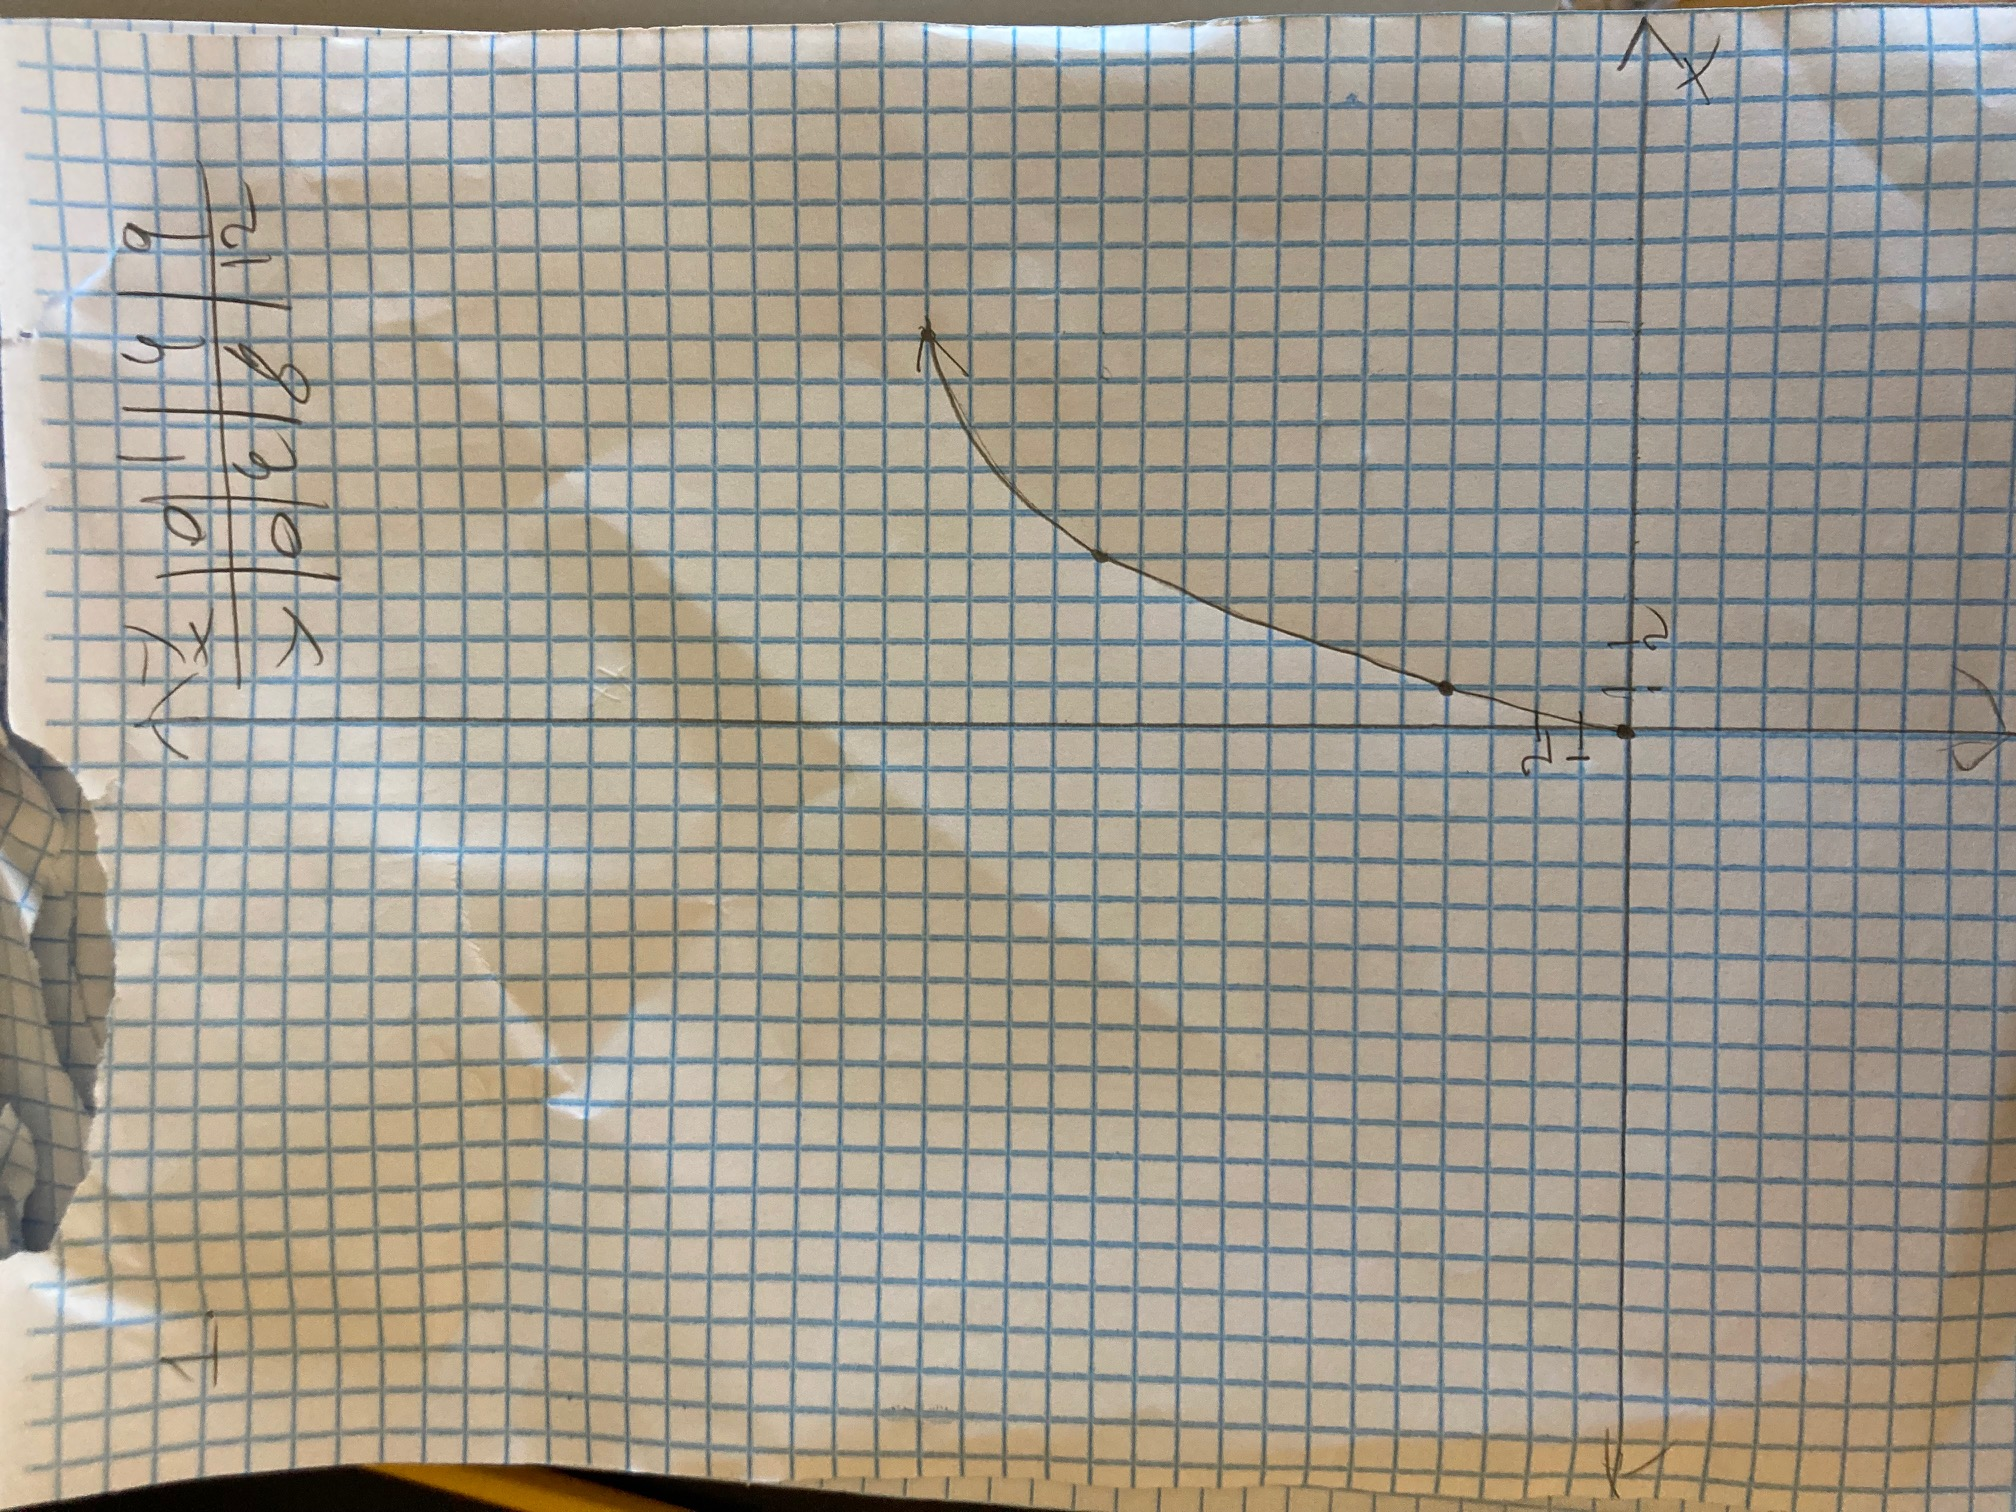
\includegraphics[width = 4in, height = 4in, angle=-90]{1} \newline
The domain of the function is $x\ge 0$, as we cannot take negative square roots. Thus, the range is $y\ge 4\sqrt{0}=0$.

\section*{3}
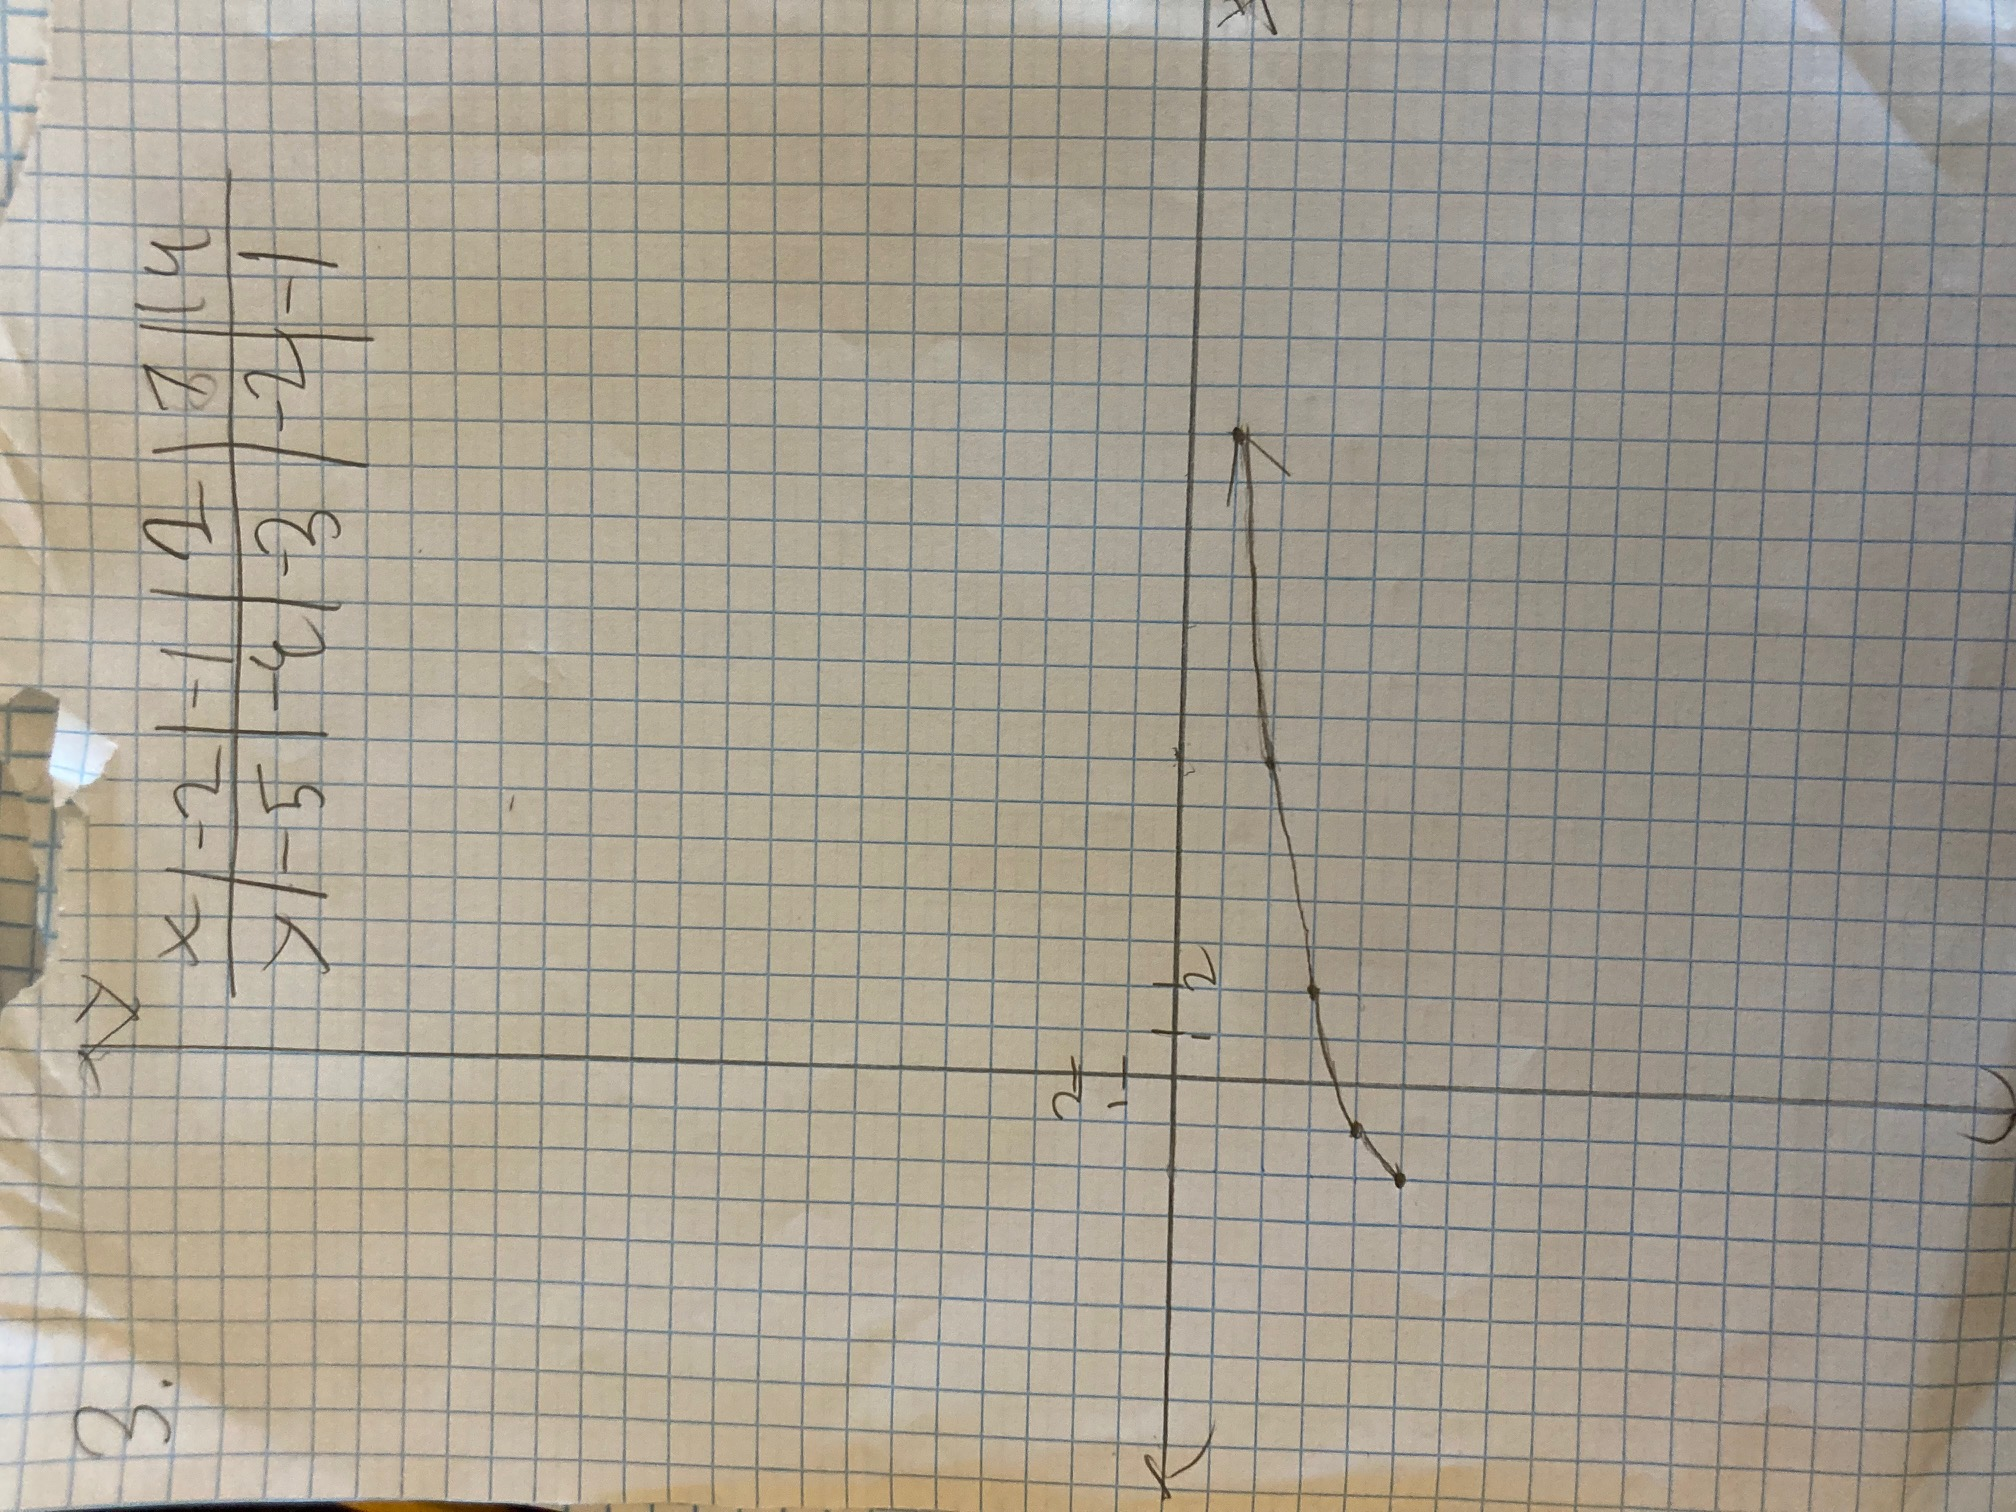
\includegraphics[width = 4in, height = 4in, angle=-90]{3} \newline
The domain of the function is $x\ge -2$, as we cannot take negative square roots (as this would happen if $\sqrt{x+2}$ is taken where 
$x<-2$). The range of the function is thus $y\ge \sqrt{0}-5=-5$.

\section*{4}
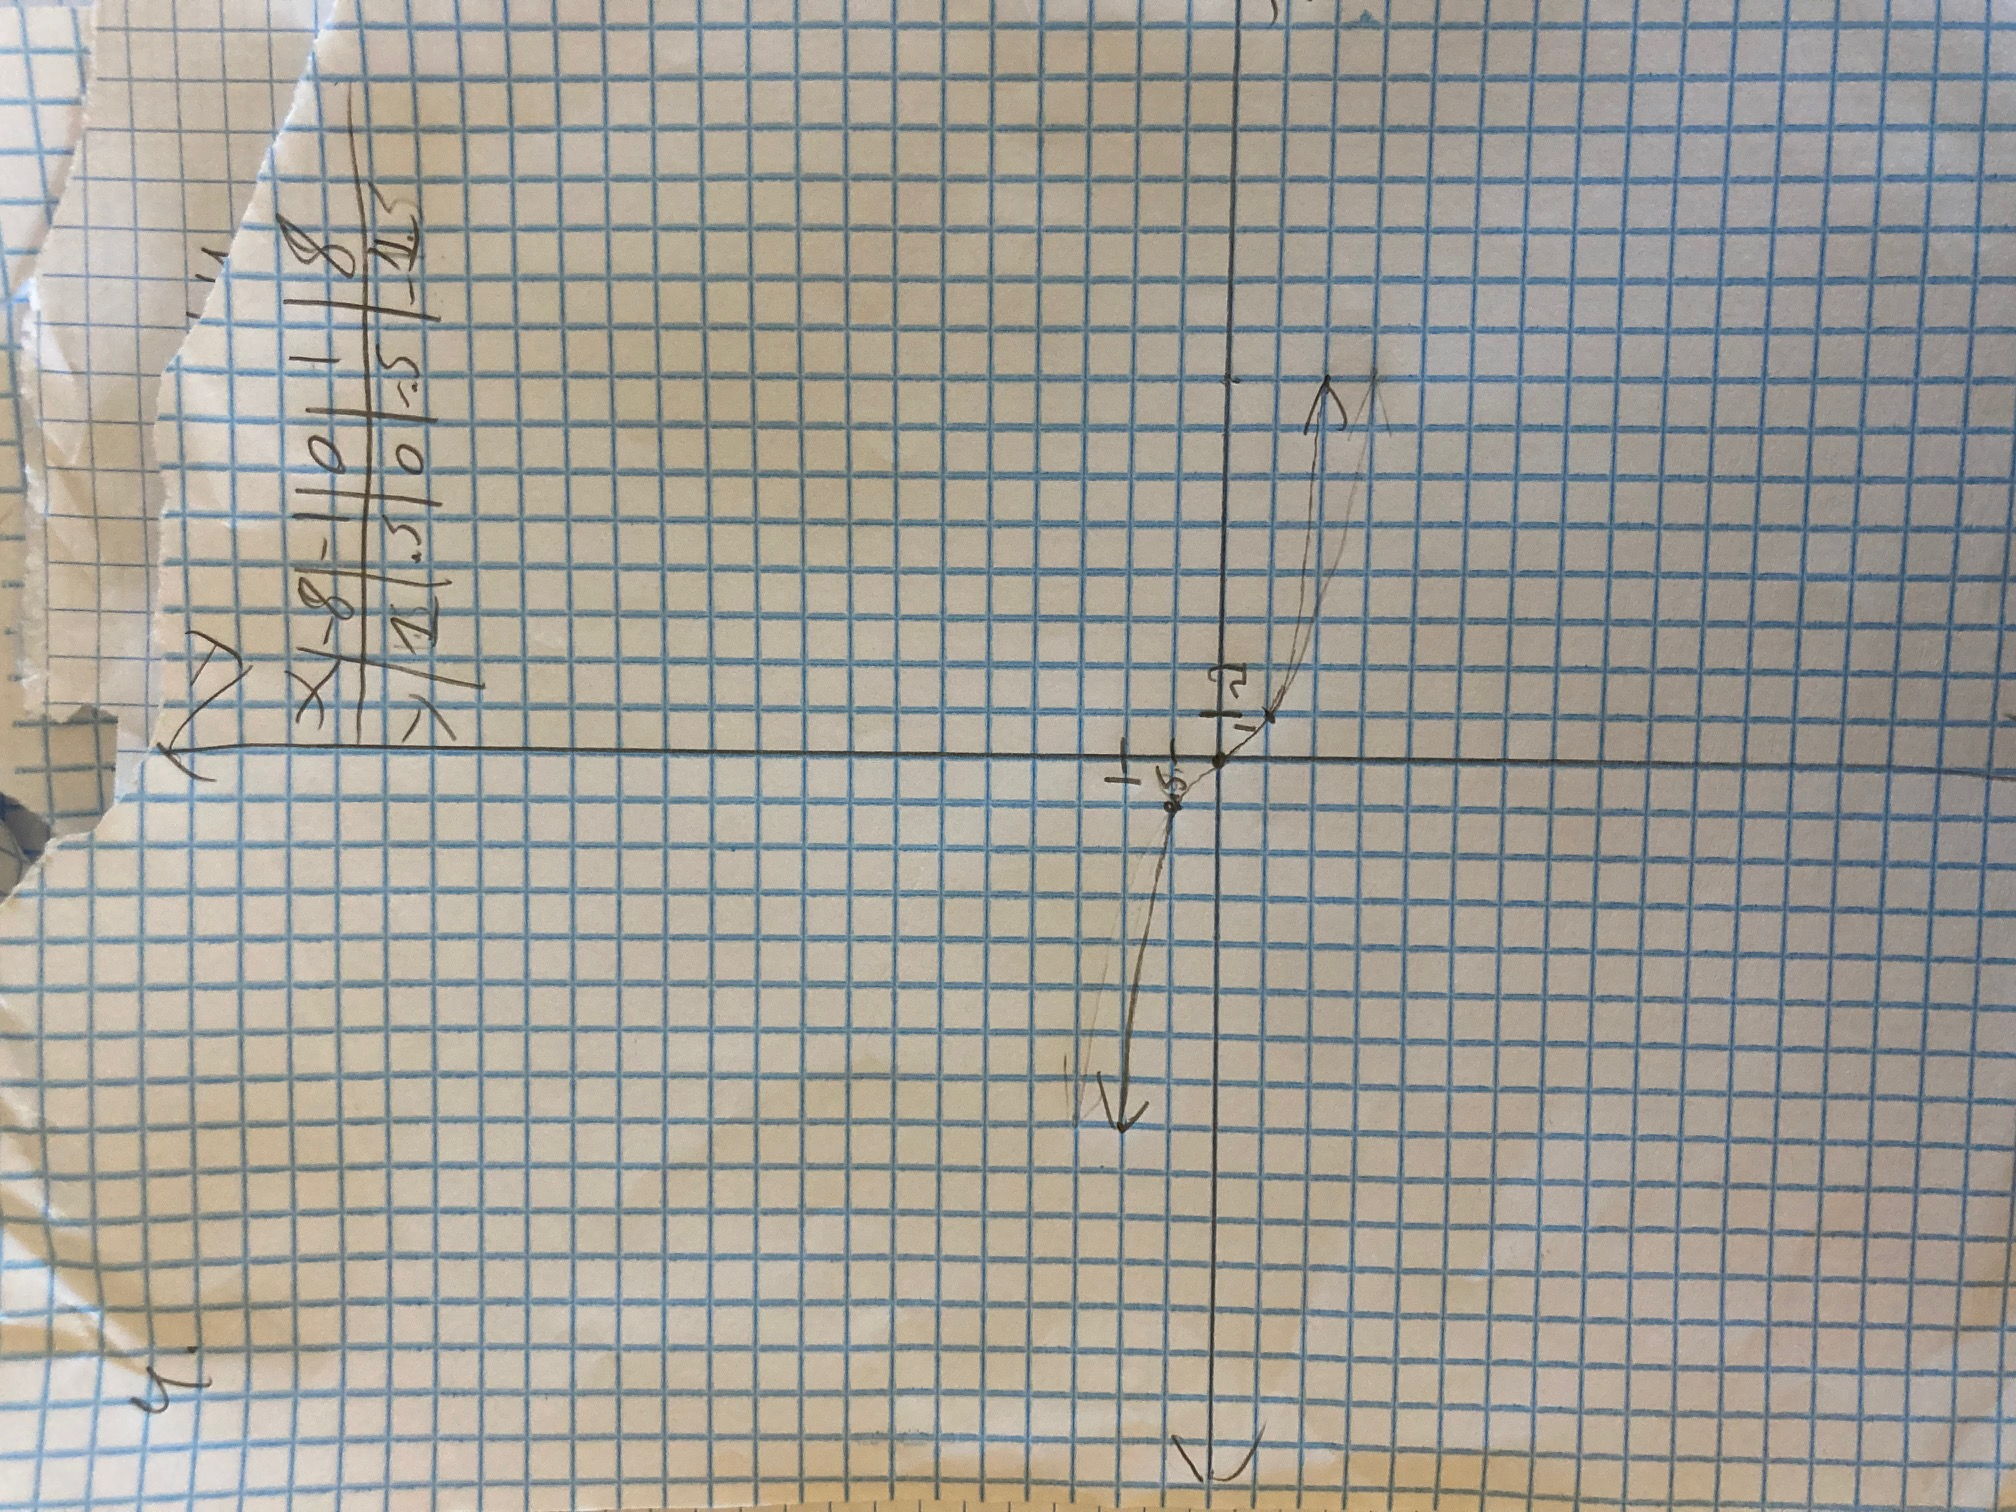
\includegraphics[width = 4in, height = 4in, angle=-90]{4}
\newline Both the domain and range of the function is all real numbers.

\section*{6}
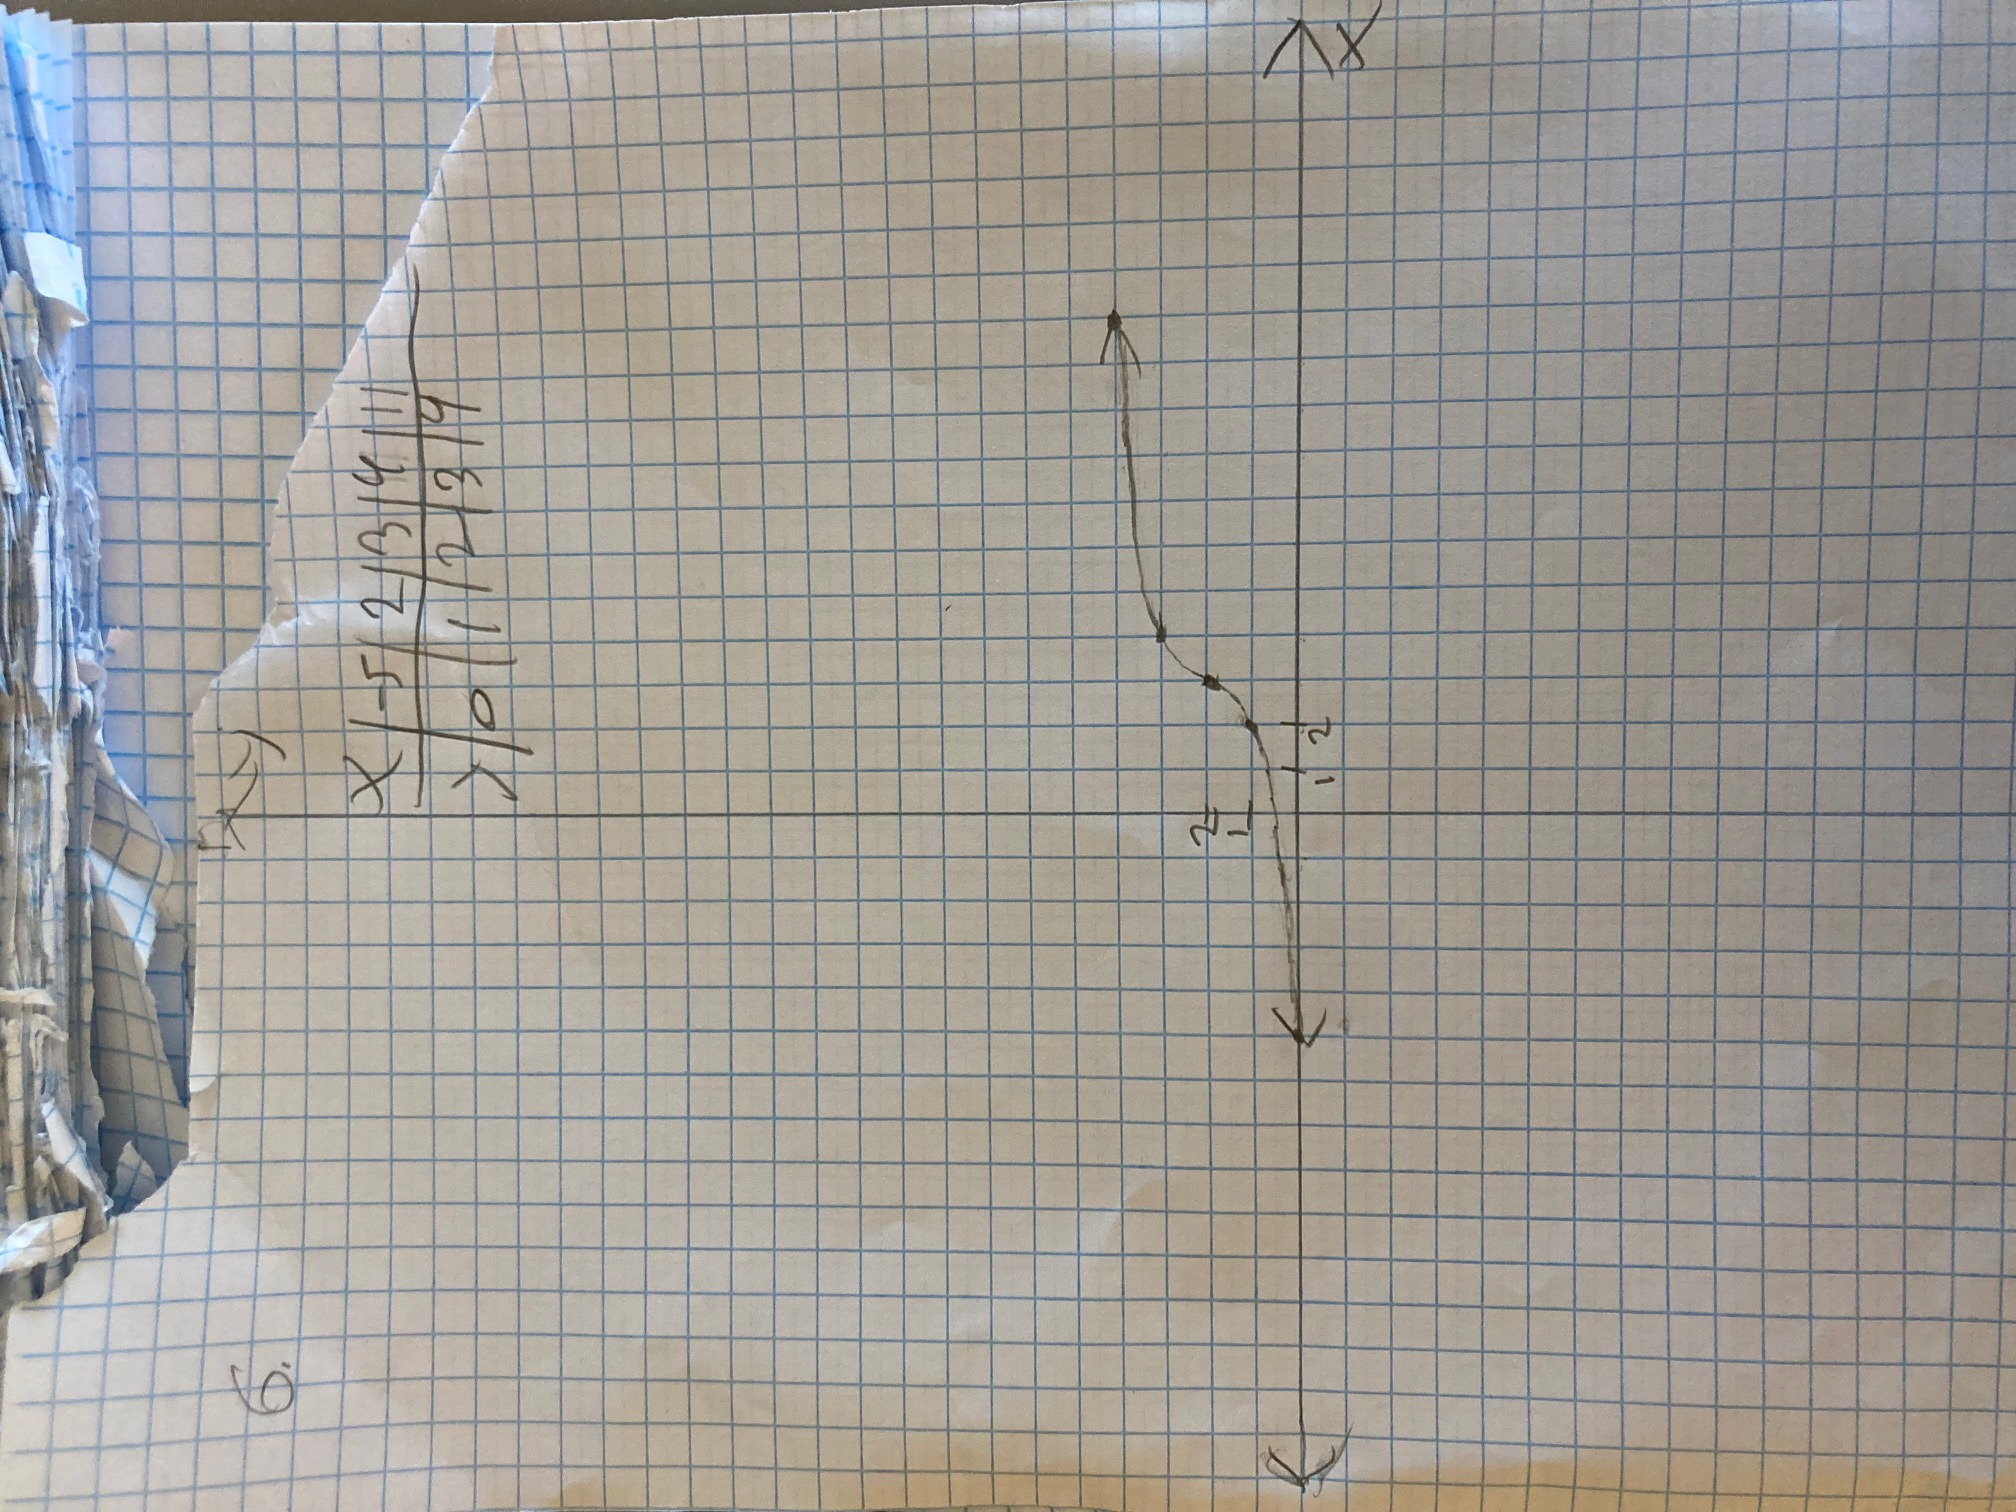
\includegraphics[width = 4in, height = 4in, angle=-90]{6}
\newline Both the domain and range of the function is all real numbers.

\section*{7}
\[ \sqrt{6x+15}=9 \] \[ 6x+15=81 \] \[ 6x=66 \] \[ x=11 \]
Check for extraneous solutions:
\[ \sqrt{6(11)+15}\? 9 \]
\[ 9=9 \]

\section*{8}
\[ \frac{1}{4}(7x+8)^\frac{3}{2}=54 \]
\[ (7x+8)^\frac{3}{2}=216 \]
\[ 7x+8=216^\frac{2}{3} \]
\[ 7x+8=(6^3)^\frac{2}{3} \]
\[ 7x+8=36 \]
\[ x=4 \]
Check for extraneous solutions:
\[ \frac{1}{4}(7(4)+8)^\frac{3}{2}\? 54 \]
\[ \frac{1}{4}(216)\? 54 \]
\[ 54=54 \]

\section*{9}
\[ \sqrt[3]{3x+5}+2=5 \]
\[ \sqrt[3]{3x+5}=3 \]
\[ 3x+5=27 \]
\[ x=\frac{22}{3} \]
Check for extraneous solutions:
\[ \sqrt[3]{3(\frac{22}{3})+5}+2\? 5 \]
\[ \sqrt[3]{27}+2\? 5 \]
\[ 5=5 \]

\section*{10}
\[ x-3=\sqrt{10x-54} \]
\[ x^2-6x+9=10x-54 \]
\[ x^2-16x+63=0 \]
\[ (x-9)(x-7)=0 \]
\[ x=9\vee x=7 \]
Check for extraneous solutions:
\[ 9-3\?\sqrt{10(9)-54} \]
\[ 6\?\sqrt{36} \]
\[ 6=6 \]
and \[ 7-3\?\sqrt{10(7)-54} \]
\[ 4\?\sqrt{16} \]
\[ 4=4 \]
meaning both $9$ and $7$ are solutions.

\section*{11}
\[ \sqrt{4x-4}=\sqrt{5x-1}-1 \]
\[ 4x-4=5x-1-2\sqrt{5x-1}+1 \]
\[ -x-4=-2\sqrt{5x-1} \]
\[ x^2+8x+16=4(5x-1) \]
\[ x^2+8x+16=20x-4 \]
\[ x^2-12x+20=0 \]
\[ (x-10)(x-2)=0 \]
\[ x=10\vee x=2 \]
Check for extraneous solutions:
\[ \sqrt{4(10)-4}\?\sqrt{5(10)-1}-1 \]
\[ \sqrt{36}\?\sqrt{49}-1 \]
\[ 6=6 \]
and \[ \sqrt{4(2)-4}\?\sqrt{5(2)-1}-1 \]
\[ \sqrt{4}\?\sqrt{9}-1 \]
\[ 2=2 \]
meaning both $10$ and $2$ are solutions.

\section*{12}
\[ \sqrt[3]{\frac{4}{5}x-9}=\sqrt[3]{x-6} \]
\[ \frac{4}{5}x-9=x-6 \]
\[ \frac{1}{5}x+3=0 \]
\[ x=-15 \]
Check for extraneous solutions:
\[ \sqrt[3]{\frac{4}{5}(-15)-9}\? \sqrt[3]{-15-6} \]
\[ \sqrt[3]{-21}=\sqrt[3]{-21} \]

\section*{13}
Suppose $P=1.88$. Thus:
\[ 1.88=0.199a^\frac{3}{2} \]
\[ \frac{1.88}{0.199}=a^\frac{3}{2} \]
\[ (\frac{1.88}{0.199})^\frac{2}{3}=a \]
\[ a\approx 4.47 \] million kilometers.

\end{document}
